% Template de présentation Beamer - Risque Systémique
\documentclass[aspectratio=169]{beamer}

% Packages nécessaires
\usepackage[french]{babel}
\usepackage[utf8]{inputenc}
\usepackage{amsmath, amssymb, amsfonts}
\usepackage{graphicx}
\usepackage{xcolor}
\usepackage{tikz}
\usepackage{booktabs}
\usepackage{natbib}

% Définition des couleurs
\definecolor{inriared}{RGB}{192, 32, 38}
\definecolor{beige}{RGB}{250, 245, 225}
\definecolor{darkblue}{RGB}{0, 51, 102}

% Configuration du thème
\usetheme{default}
\usecolortheme{default}
\setbeamercolor{background canvas}{bg=beige}
\setbeamercolor{title}{fg=inriared}
\setbeamercolor{frametitle}{fg=darkblue}
\setbeamercolor{structure}{fg=darkblue}
\setbeamercolor{normal text}{fg=black}
\setbeamercolor{itemize item}{fg=inriared}
\setbeamercolor{itemize subitem}{fg=inriared}

% Police plus fine
\usefonttheme{professionalfonts}
\setbeamerfont{normal text}{size=\normalsize}
\setbeamerfont{itemize/enumerate body}{size=\normalsize}
\setbeamerfont{itemize/enumerate subbody}{size=\normalsize}



% Style des titres de slides
\setbeamerfont{frametitle}{size=\large\bfseries}
\setbeamertemplate{frametitle}{
    \vspace*{0.1cm}
    \insertframetitle
    \vspace{0.07cm}
    \begin{tikzpicture}
        \draw[inriared, thick] (0,0) -- (\textwidth,0);
    \end{tikzpicture}
}

% Pied de page personnalisé
\setbeamertemplate{footline}{
    \begin{beamercolorbox}[wd=\paperwidth,ht=2.5ex,dp=1.125ex,leftskip=.5cm,rightskip=.5cm]{footline}
        \hfill \insertframenumber\ / \inserttotalframenumber
    \end{beamercolorbox}
}

% En-tête avec logos
\addtobeamertemplate{frametitle}{}{
    \begin{tikzpicture}[remember picture,overlay]
        \node[anchor=north east] at ([shift={(-0.4cm,-0.4cm)}]current page.north east) {
\includegraphics[height=0.5cm]{RF-INria_Bloc-marque}};
    \end{tikzpicture}
}

% Informations sur la présentation
\title{\large Risque systémique vu comme un seuil de résilience}
\subtitle{Introduction à la Recherche en Laboratoire (IRL)}
\author{Hamidou Diallo}
\institute{INRIA Grenoble, équipes DANCE et POLARIS\\ENSIMAG}
\date{13 mai 2025}

\begin{document}

% Slide de titre
    \begin{frame}
        \titlepage
        % Logos des équipes DANCE et POLARIS
        \begin{center}
            \vspace{1cm}
            
\includegraphics[height=1cm]{RF-INria_Bloc-marque}
        \end{center}
    \end{frame}

% Sommaire
    \begin{frame}{Plan de la présentation}
        \tableofcontents
    \end{frame}

% ======= SECTION 1 =======
    \section{Contexte et collaboration}\label{sec:contexte-et-collaboration}
    \begin{frame}{Contexte et collaboration}
        \begin{columns}
            \begin{column}{0.6\textwidth}
                \begin{itemize}
                    \item Projet IRL en collaboration avec:
                    \begin{itemize}
                        \item DANCE: Dynamiques sur réseaux
                        \item POLARIS: Systèmes distribués
                    \end{itemize}
                    \vspace{0.3cm}
                    \item Encadrants: F. Garin, P. Frasca, N. Gast
                    \vspace{0.3cm}
                    \item Approche interdisciplinaire:
                    \begin{itemize}
                        \item Théorie des graphes
                        \item Informatique
                        \item Modélisation
                    \end{itemize}
                \end{itemize}
            \end{column}
            \begin{column}{0.4\textwidth}
                \centering
                
\includegraphics[width=0.65\linewidth]{RF-INria_Bloc-marque}
                \vspace{0.3cm}

                \small Une demi-journée/semaine\\pendant 3 mois
            \end{column}
        \end{columns}
    \end{frame}

% ======= SECTION 2 =======
    \section{Risque systémique et crises financières}\label{sec:risque-systemique-et-crises-financieres}
    \begin{frame}{Risque systémique et son importance}
        \begin{itemize}
            \item \textbf{Risque systémique}: Probabilité qu'une proportion importante de banque du système financier face défaut.
            \vspace{0.3cm}
            \item \textbf{Exemple}: Crise de 2007-2008, faillite de Lehman Brothers
            \vspace{0.3cm}
            \item \textbf{Question centrale}:
            \begin{itemize}
                \item Les interconnexions réduisent-elles ou amplifient-elles l'impact d'un choc?
                \item Existe-t-il un seuil critique?
            \end{itemize}
        \end{itemize}

    \end{frame}

    \begin{frame}{État de l'art}
        \begin{itemize}
            \item Peter Young ~\cite{peyton2016contagion} pour une synthèse de l'état de l'art en reseau financier.
            \item ~\cite{jglass2006topologyus} pour la Topologie des réseaux interbancaires.
            \item ~\cite{nier2008stability} pour les idées de simulation et pour l'interpretation des résulats.
            \item ~\cite{eisenberg2001systemic} Eisenberg et Noe pour son algorithme.
        \end{itemize}
    \end{frame}

% ======= SECTION 3 =======
    \section{Formalisation du problème}\label{sec:formalisation-du-probleme}
    \begin{frame}{Modélisation du réseau interbancaire}
        \begin{itemize}
            \item \textbf{Banque $i$}:
            \begin{itemize}
                \item $c_i$: actifs extérieurs (prêts aux entités externes)
                \item $b_i$: passifs extérieurs (emprunts auprès d'entités externes)
                \item $[I]_{ij}$: obligation de $i$ envers $j$
            \end{itemize}
            \vspace{0.2cm}
            \item \textbf{Réseau interbancaire}: graphe orienté pondéré $(R,I,c,b)$
            \begin{itemize}
                \item $R$: graphe d'Erdös-Rényi avec probabilité $p$ de connexion
                \item $I$: matrice d'obligations entre banques
            \end{itemize}
            \vspace{0.2cm}
            \item \textbf{Défaut}: Valeur nette négative
        \end{itemize}
    \end{frame}

    \begin{frame}{Exemple de propagation de défaut}
        \begin{figure}[htbp]
            \centering
            \begin{tikzpicture}[
                bank/.style={circle, draw, thick, minimum size=0.9cm, font=\footnotesize},
                obligation/.style={font=\footnotesize, ->, >=latex},
                external/.style={font=\footnotesize, ->, >=latex},
                networth/.style={font=\footnotesize, text=blue}
            ]
                % Définir les banques (nœuds) - espacement réduit
                \node[bank] (B1) at (0,0) {A};
                \node[bank] (B2) at (4,0) {B};
                \node[bank] (B3) at (0,-3) {D};
                \node[bank] (B4) at (4,-3) {C};

                % Net worth sous chaque banque
                \node[networth] at (0,-0.8) {10};
                \node[networth] at (4,-0.8) {10};
                \node[networth] at (0,-3.8) {4};
                \node[networth] at (4,-3.8) {10};

                % Définir les obligations interbancaires (lignes droites)
                \draw[obligation] (B1) to node[midway, above] {180} (B2);
                \draw[obligation] (B2) to node[pos=0.35, right=2pt] {100} (B4);
                \draw[obligation] (B4) to node[midway, below] {100} (B3);
                \draw[obligation] (B3) to node[pos=0.65, left=2pt] {150} (B1);
                \draw[obligation] (B4) to node[pos=0.65, left=2pt] {100} (B1);

                % Actifs externes (flèches entrantes en pointillé)
                \node[font=\footnotesize] (EA1) at (-1.5,0) {$c_1$};
                \node[font=\footnotesize] (EA2) at (5.5,0) {$c_2$};
                \node[font=\footnotesize] (EA3) at (-1.5,-3) {$c_3$};
                \node[font=\footnotesize] (EA4) at (5.5,-3) {$c_4$};

                \draw[external] (EA1) to node[midway, above] {120} (B1);
                \draw[external] (EA2) to node[midway, above] {30} (B2);
                \draw[external] (EA3) to node[midway, above] {204} (B3);
                \draw[external] (EA4) to node[midway, above] {160} (B4);

                % Passifs externes (flèches sortantes en pointillé)
                \node[font=\footnotesize] (EP1) at (-1.2,-1) {$b_1$};
                \node[font=\footnotesize] (EP2) at (5.2,-1) {$b_2$};
                \node[font=\footnotesize] (EP3) at (-1.2,-4) {$b_3$};
                \node[font=\footnotesize] (EP4) at (5.2,-4) {$b_4$};

                \draw[external] (B1) to node[midway, above] {180} (EP1);
                \draw[external] (B2) to node[midway, above] {100} (EP2);
                \draw[external] (B3) to node[midway, above] {150} (EP3);
                \draw[external] (B4) to node[midway, above] {50} (EP4);
            \end{tikzpicture}
            \caption{Réseau interbancaire avec actifs et passifs externes}
            \label{fig:network_with_externals}
        \end{figure}

        \begin{center}
            \small Comment calculer les paiements d'équilibre lors d'une cascade de défauts?
        \end{center}
    \end{frame}

% ======= SECTION 4 =======
    \section{Approche par simulation}\label{sec:approche-par-simulation}
    \begin{frame}{Méthodologie de simulation}
        \begin{itemize}
            \item \textbf{Algorithme d'Eisenberg-Noe} pour la propagation des défauts
            \item \textbf{Génération de réseaux}: graphes d'Erdös-Rényi
            \begin{itemize}
                \item Probabilité $p$ d'interconnexion
                \item Loi produit avec une Gamma et une Bernouilli pour les obligations
            \end{itemize}
            \item \textbf{Choc exogène}: gravité $g = \frac{\|x\|}{\|c\|}$ (proportion d'actifs extérieurs touchés)
        \end{itemize}
    \end{frame}

    \begin{frame}{Implémentation}
        \center
        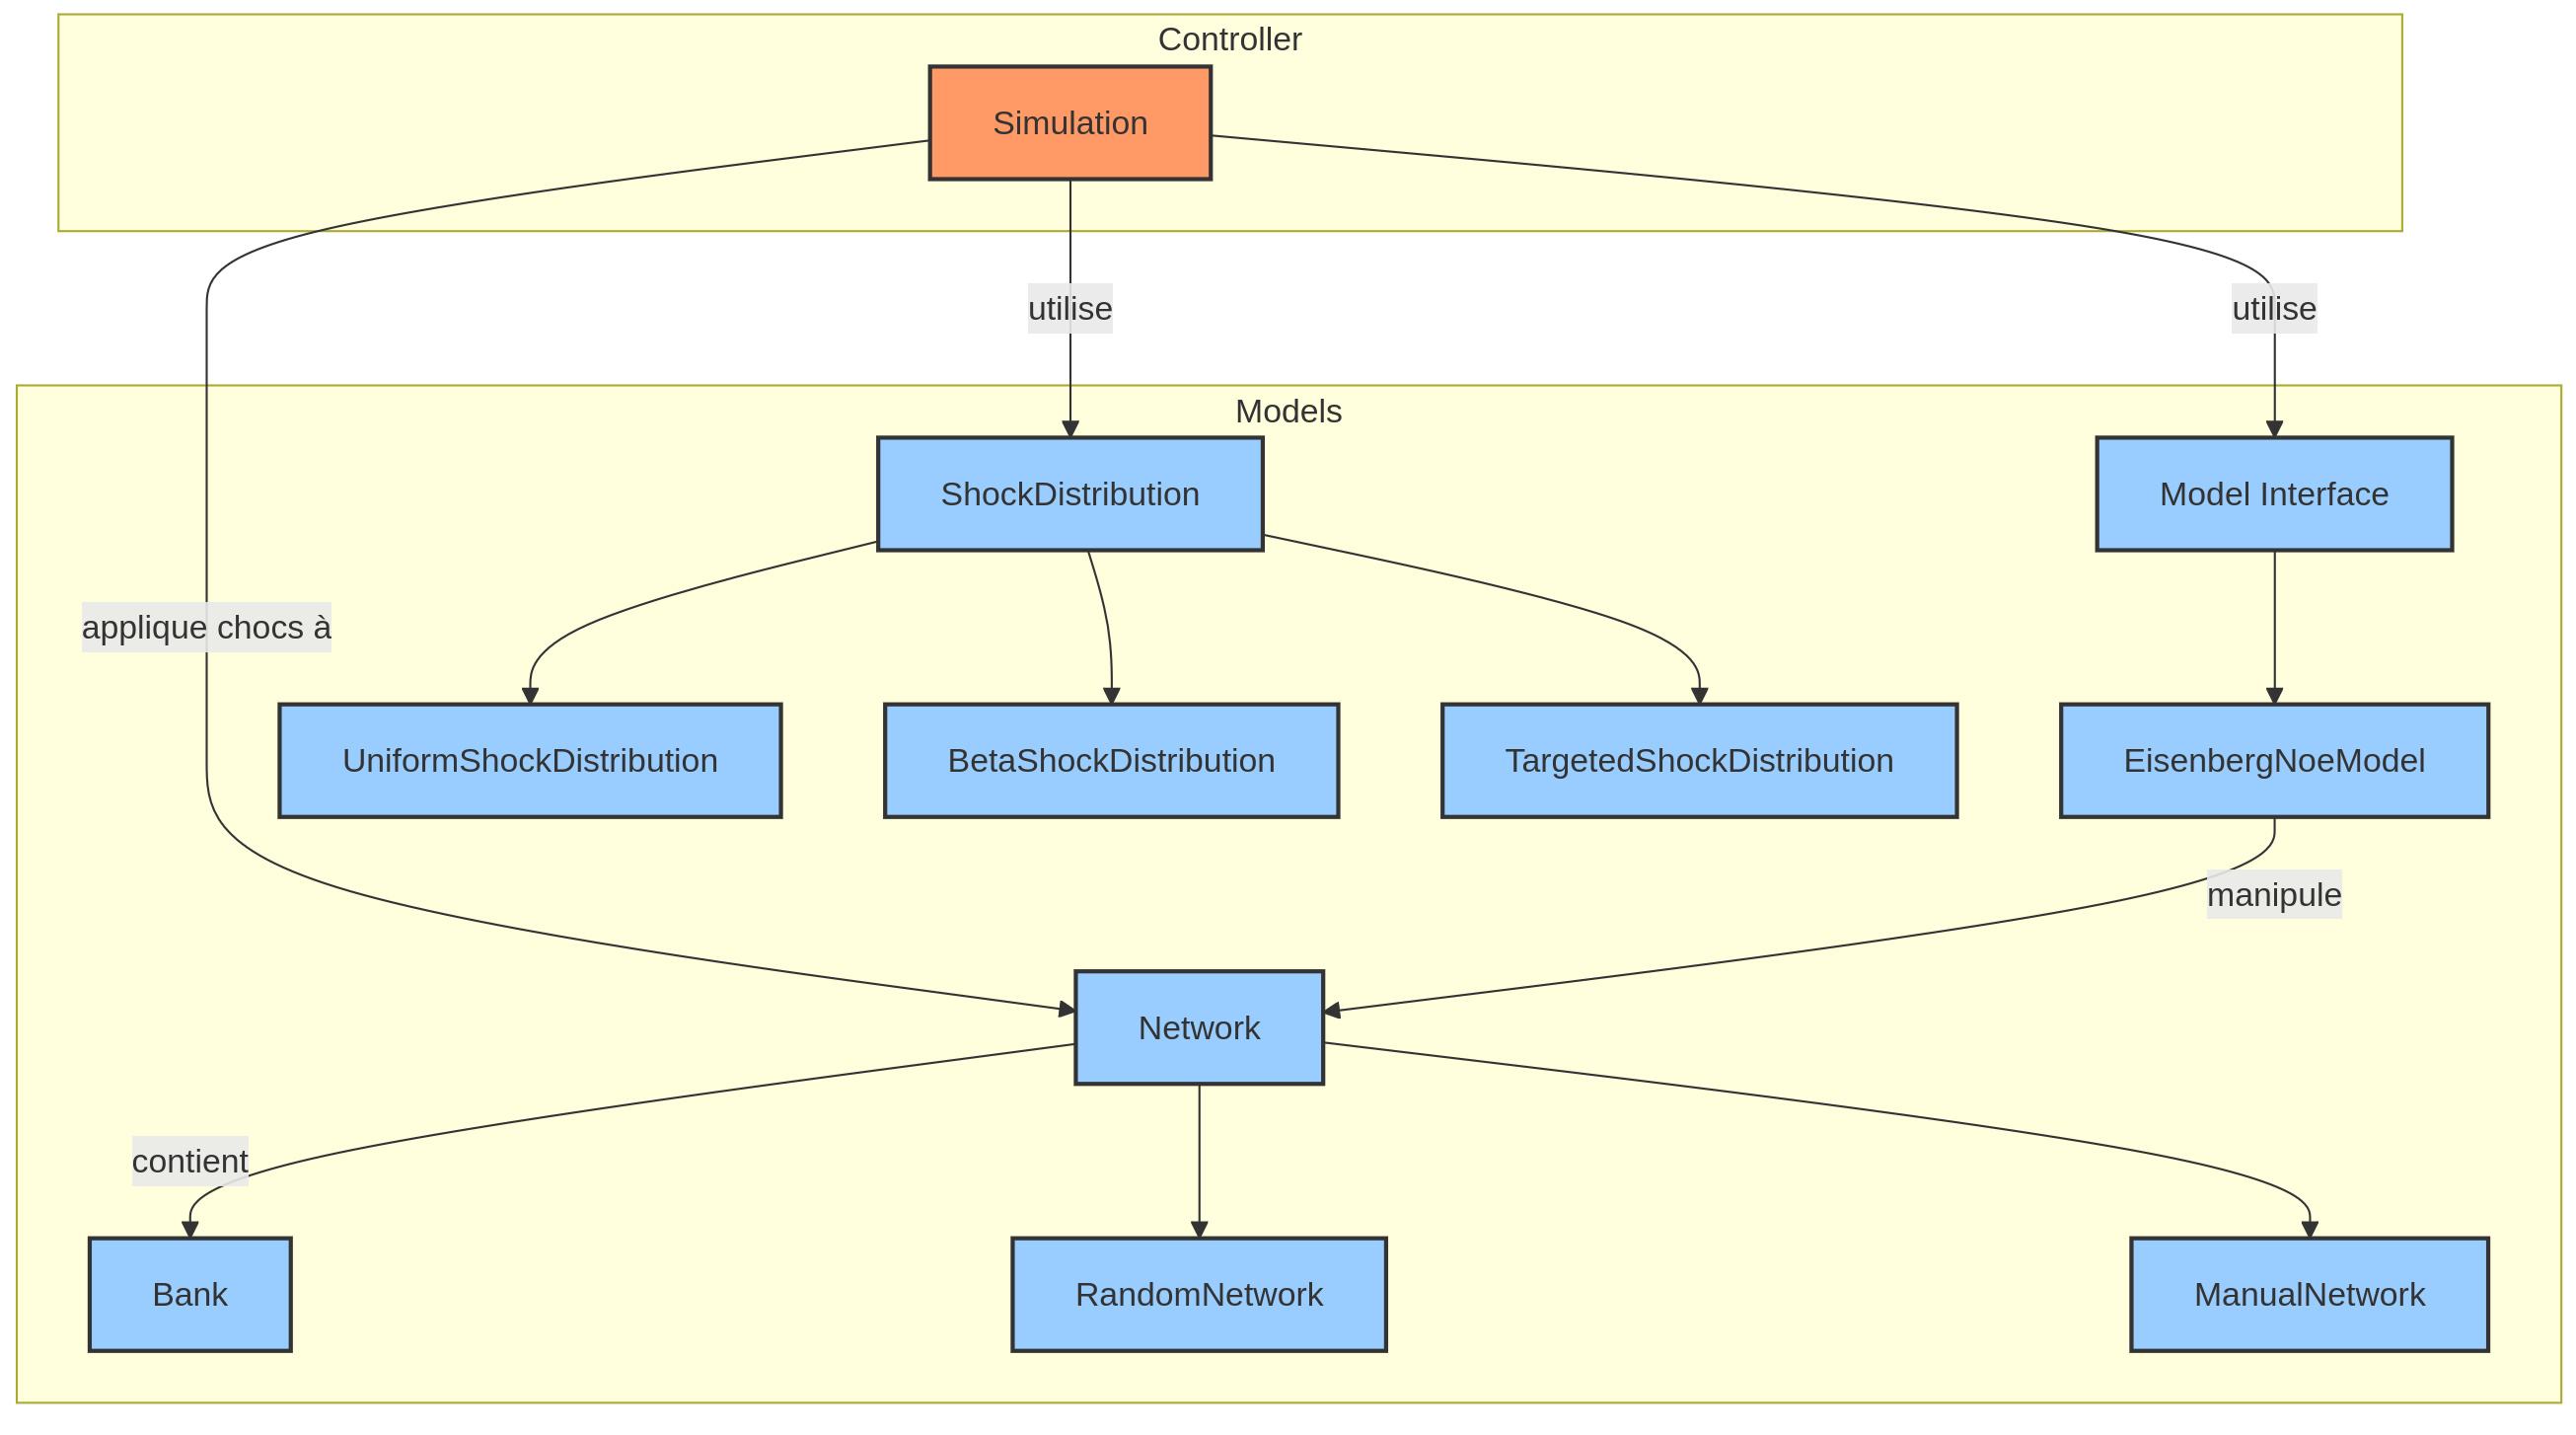
\includegraphics[width=0.75\linewidth]{diagramme uml}

        \vspace{0.01cm}
        \small Architecture MVC pour une modélisation modulaire

    \end{frame}

% ======= SECTION 5 =======
    \section{Analyse des résultats}\label{sec:analyse-des-resultats}

    \begin{frame}{Effet de la densité du réseau - Part 1}
        \begin{columns}
            \begin{column}{0.5\textwidth}
                \begin{itemize}
                    \item \textbf{Observation principale}: Les réseaux moins connectés sont plus résistants aux chocs exogènes
                    \vspace{0.1cm}
                    \item \textbf{Explication}: Moins de canaux de propagation des défauts
                \end{itemize}
            \end{column}
            \begin{column}{0.5\textwidth}
                \begin{center}
                    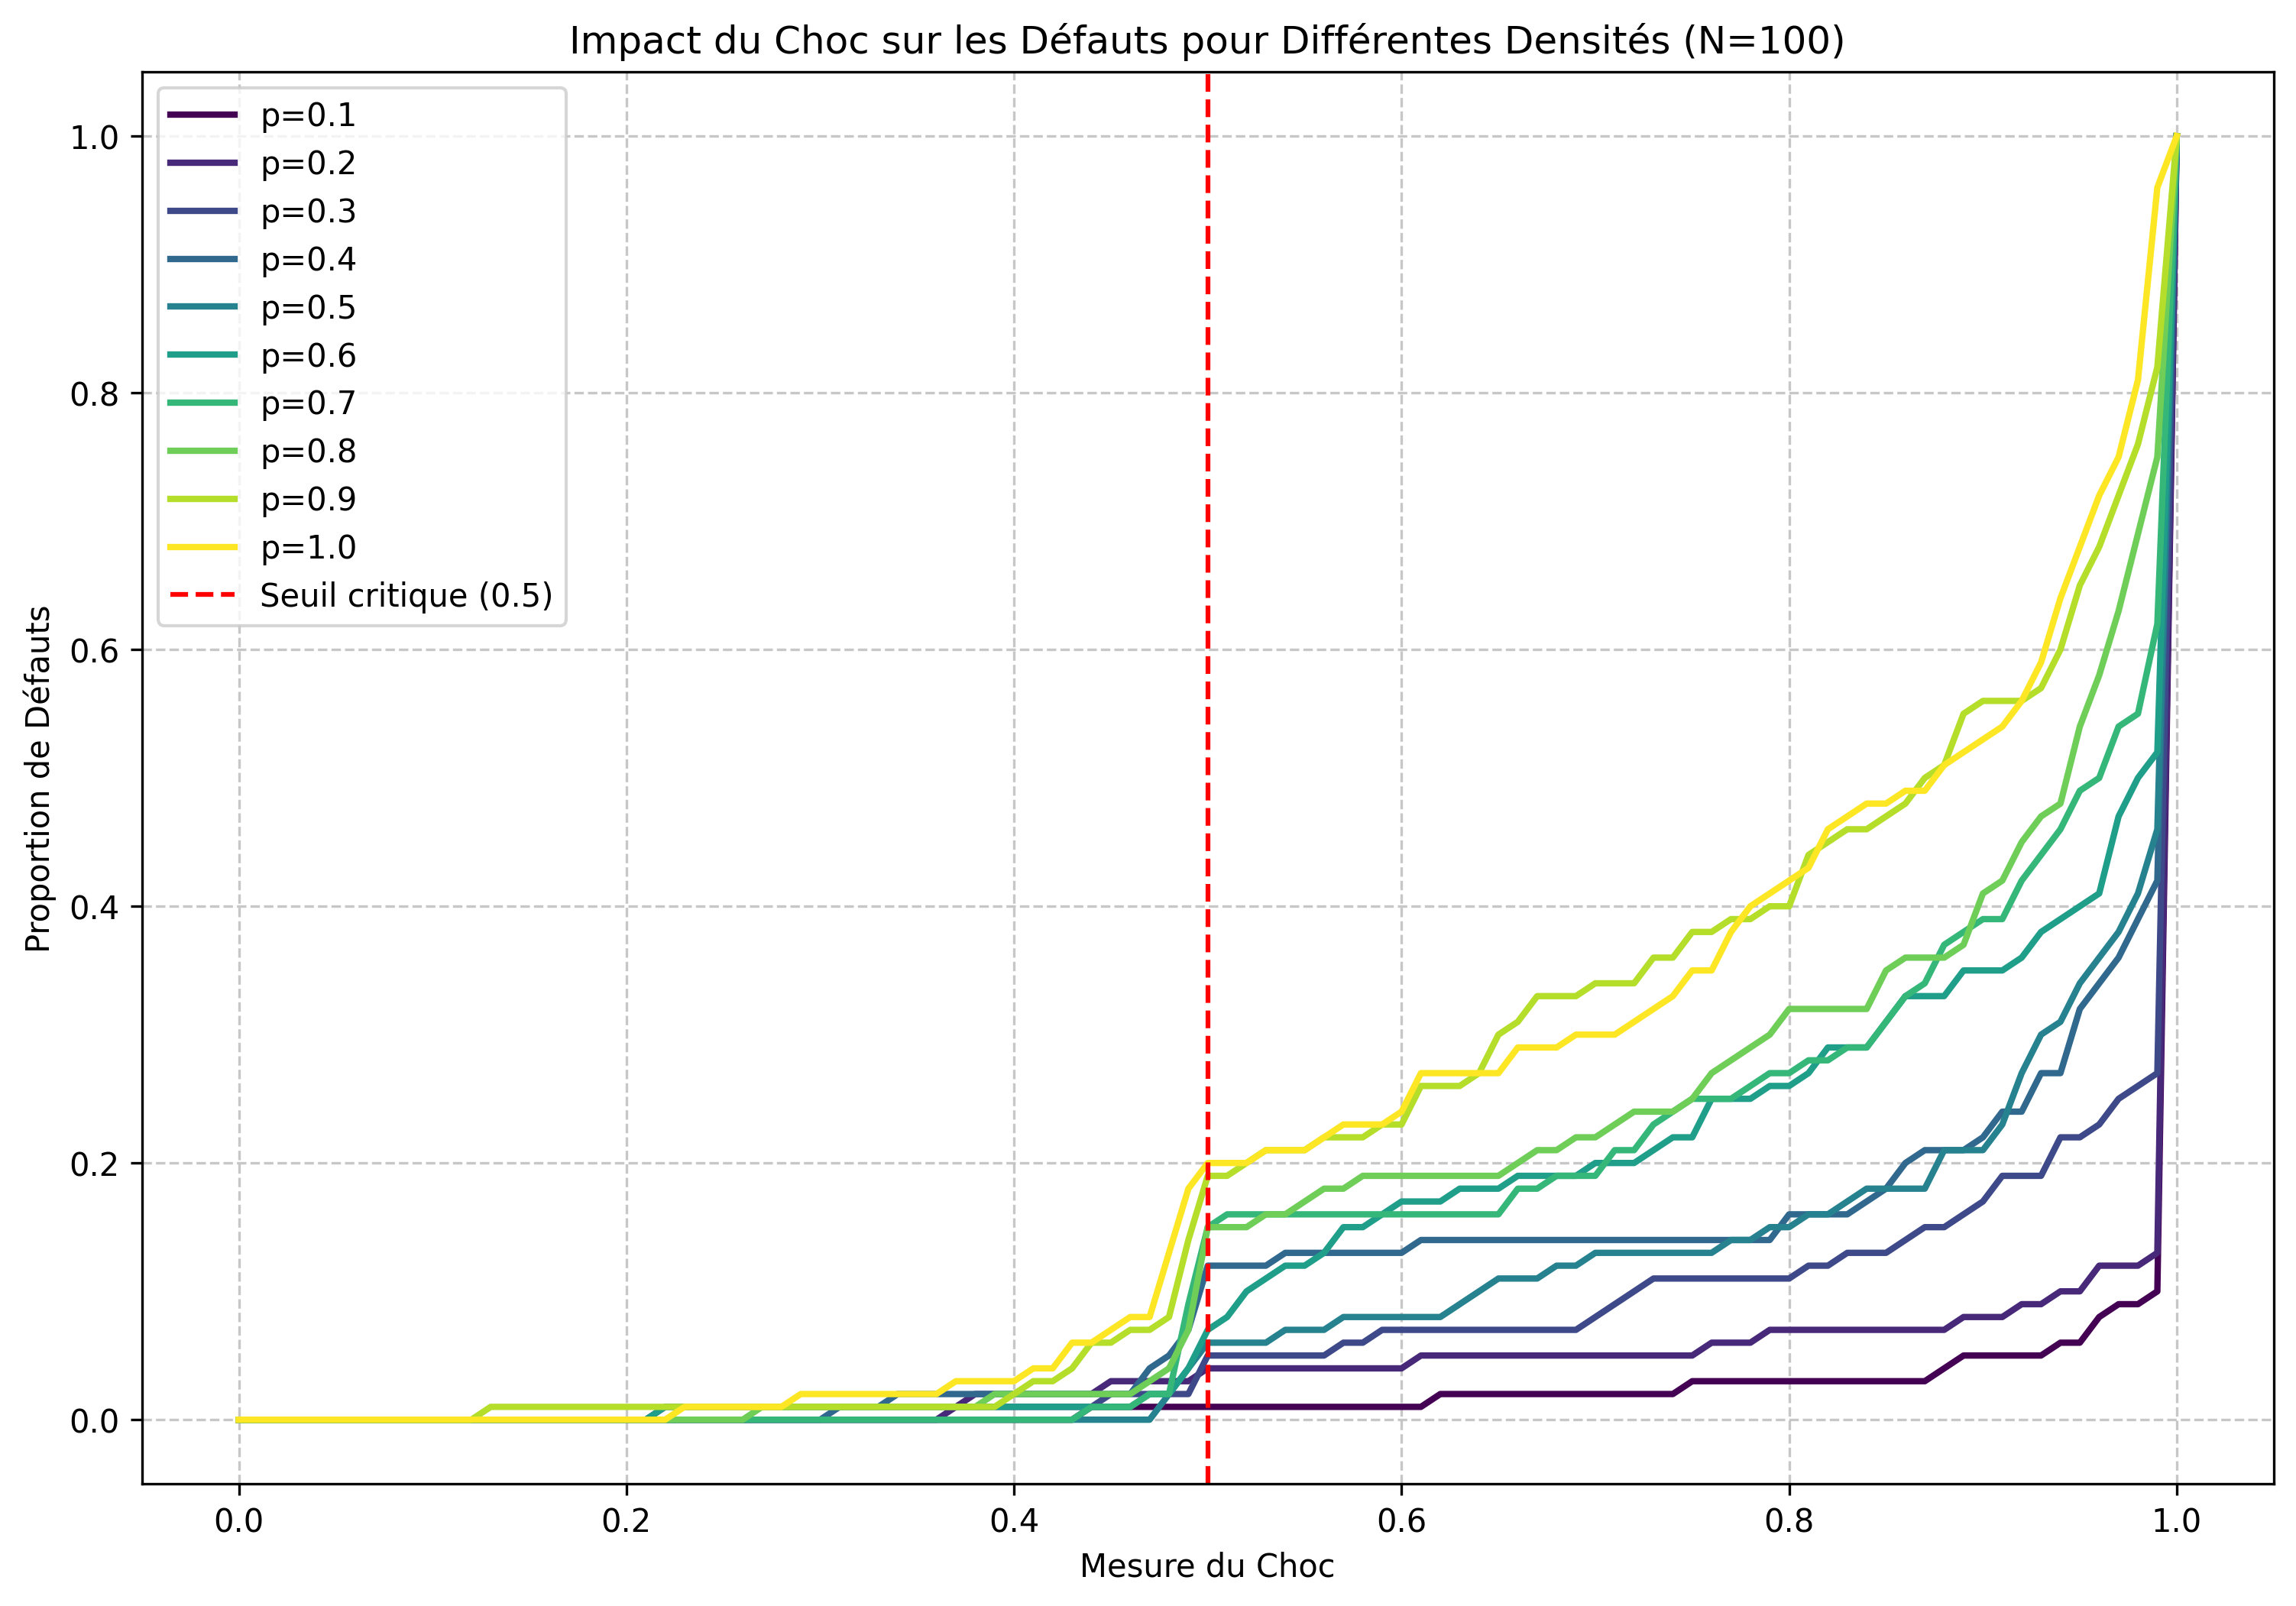
\includegraphics[width=1\linewidth]{fig2_2d_prob_shock_default}

                    \small Proportion de défauts selon la densité du réseau
                \end{center}
            \end{column}
        \end{columns}

    \end{frame}

    \begin{frame}{Observation d'un seuil critique}
        \begin{columns}
            \begin{column}{0.5\textwidth}
                    \textbf{Seuil critique} observé à $g \approx 0.5$
                    \begin{itemize}
                        \item Quand 50\% des actifs extérieurs sont touchés, le système change de régime
                    \end{itemize}
            \end{column}
            \begin{column}{0.5\textwidth}
                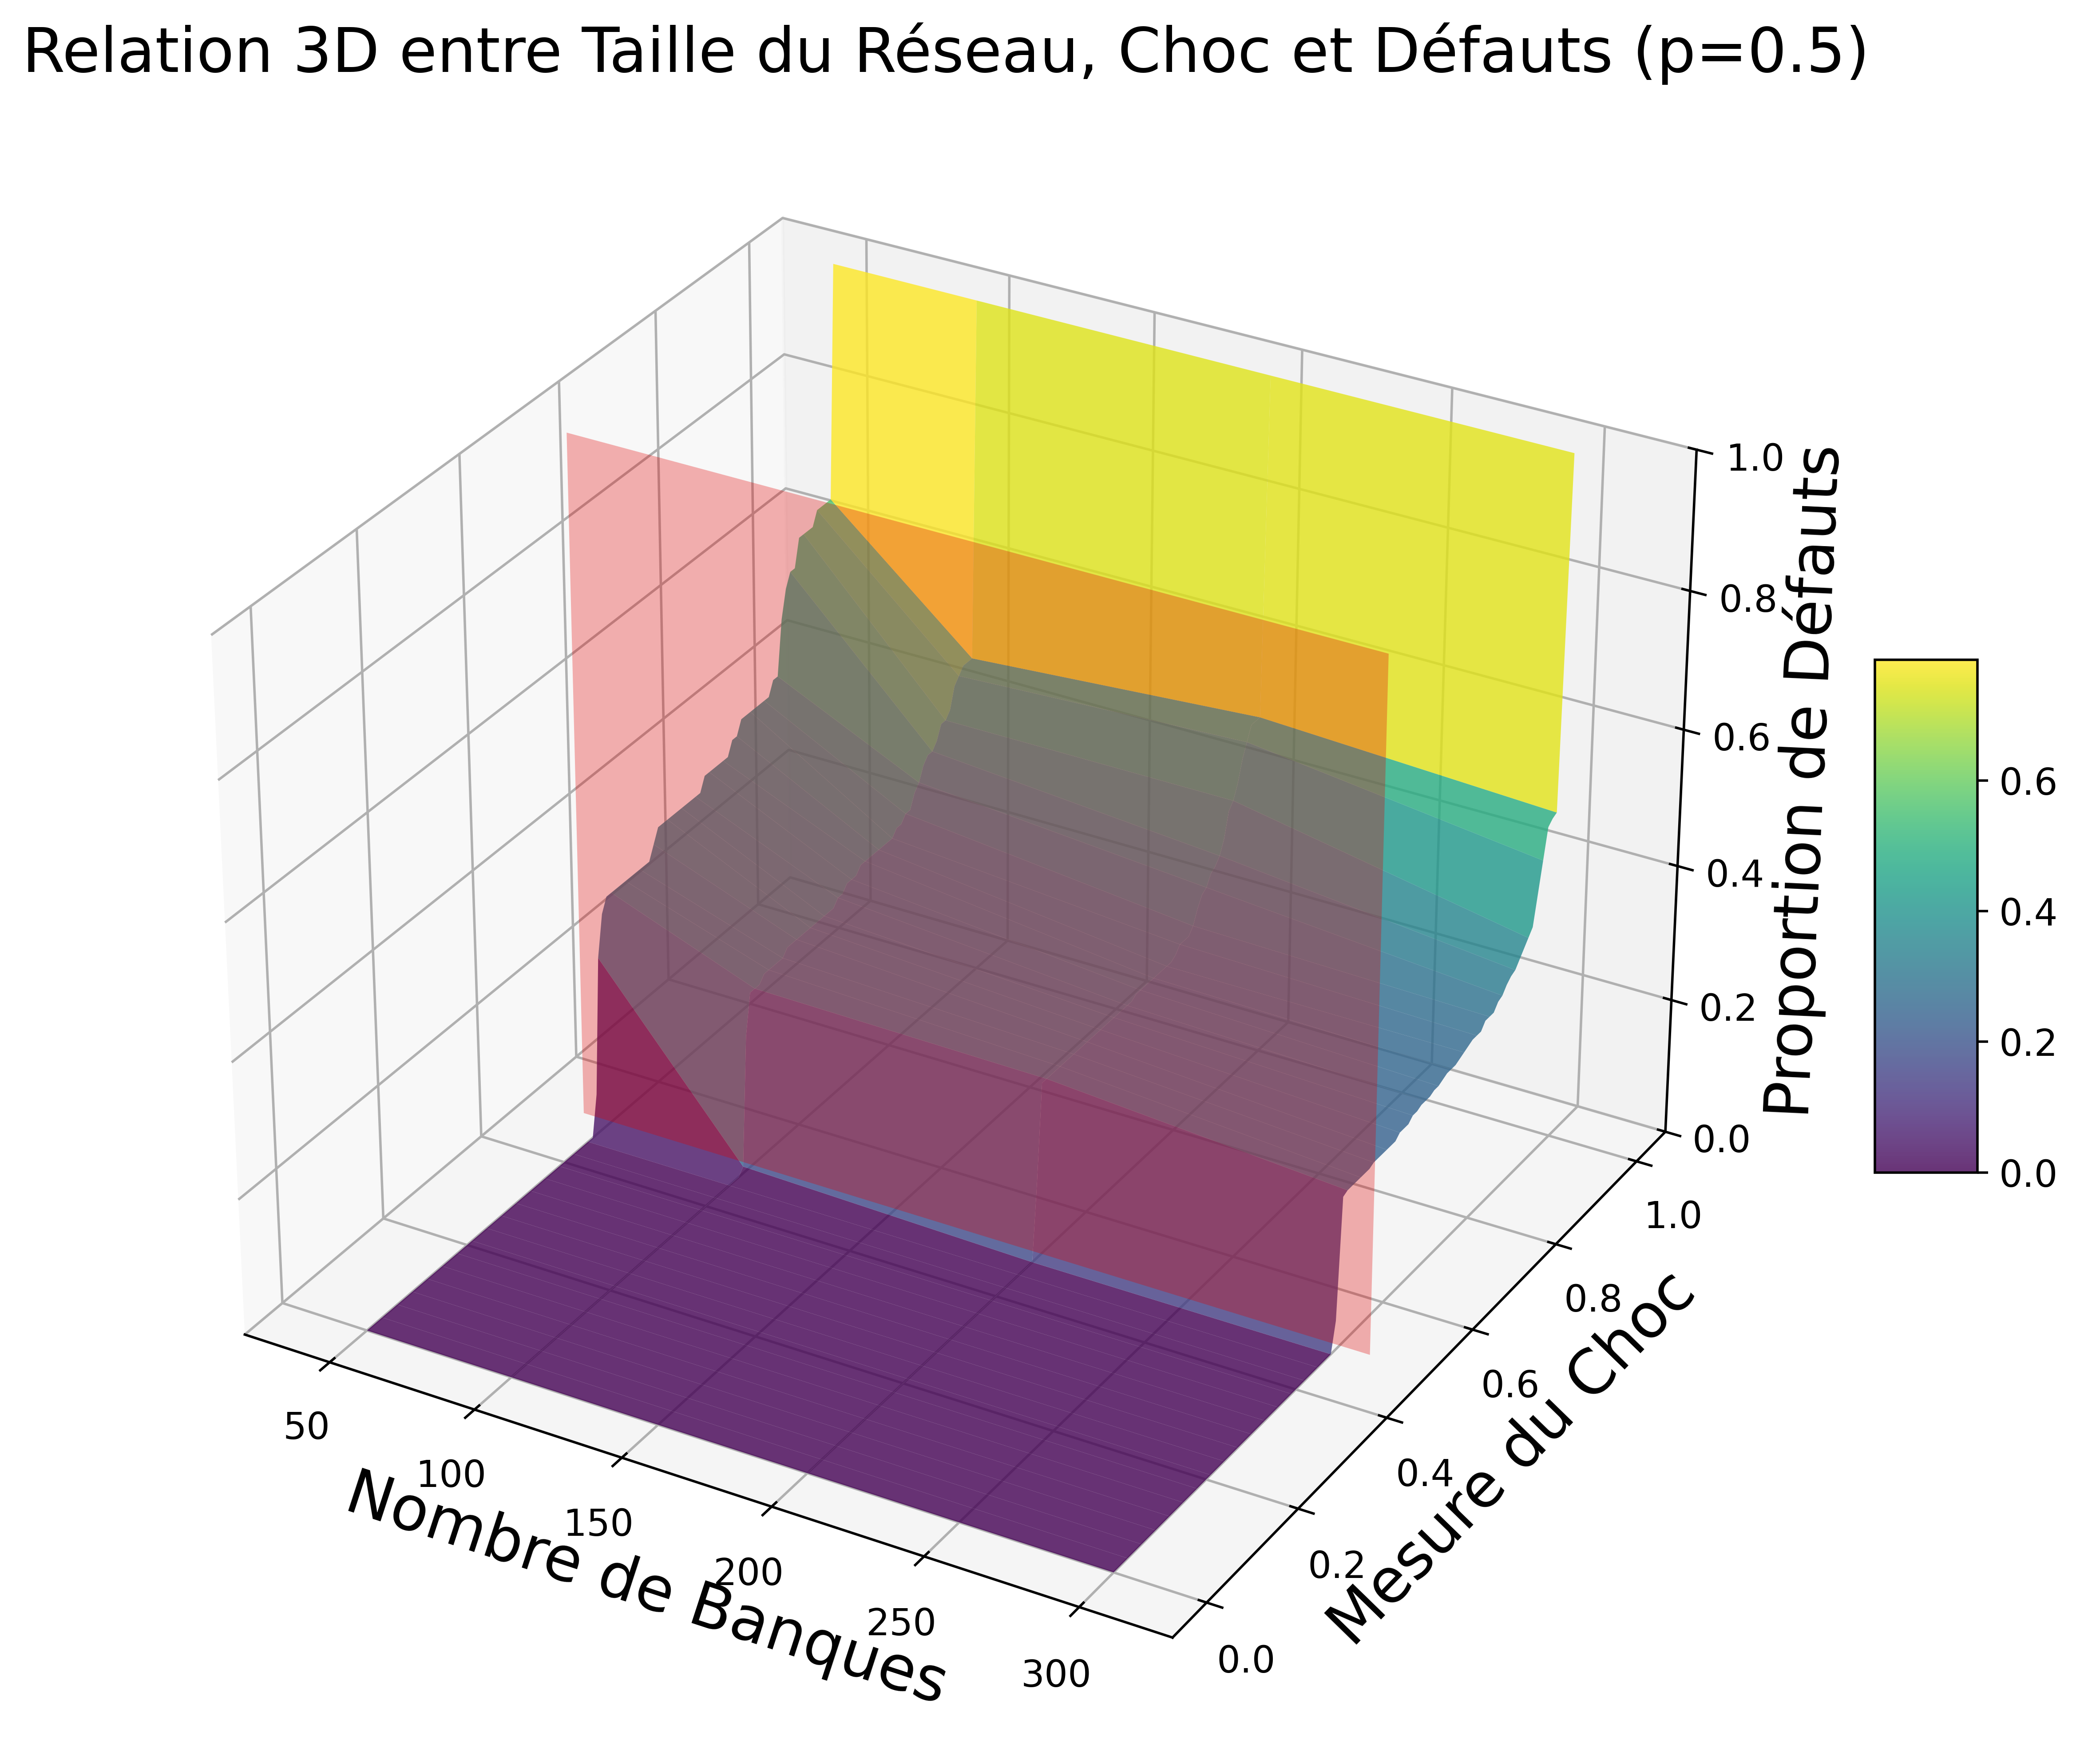
\includegraphics[width=1\linewidth]{fig1_3d_bank_shock_default}
            \end{column}
        \end{columns}

        \begin{center}
            \scriptsize \emph{→ Phénomène persistant quelle que soit la taille du réseau}\\
            \scriptsize \emph{→ Transition dans la dynamique de propagation des défauts}
        \end{center}
    \end{frame}




% ======= SECTION 6 =======
    \section{Ouverture et perspectives}\label{sec:ouverture-et-perspectives}
    \begin{frame}{Limites et perspectives de recherche}
        \begin{itemize}
            \item \textbf{Limites actuelles}:
            \begin{itemize}
                \item Topologie unique (Erdös-Rényi)
                \item Un approfondissement théorique sur le seuil à 0.5
                \item Modèle de choc simplifié
            \end{itemize}
            \vspace{0.3cm}
            \item \textbf{Perspectives}:
            \begin{itemize}
                \item Topologies alternatives: scale-free, small-world, core-periphery
                \item Analyse du rôle des cycles dans la propagation
                \item Modélisation stochastique des chocs
            \end{itemize}
        \end{itemize}
    \end{frame}

% Slide final
    \begin{frame}{Conclusion}
        \begin{center}
            \begin{itemize}
                \item \textbf{Un seuil critique observé à 50\%} du choc exogène
                \item \textbf{Les réseaux moins denses sont plus résistants} aux chocs systémiques
            \end{itemize}

            \vspace{1cm}
            Merci de votre attention!

            \vspace{0.5cm}
            \small
            Code source: \url{https://github.com/hamidou1089-1/}\\
            Contact: \href{mailto:hamidou.diallo@grenoble-inp.org}{hamidou.diallo@inria.fr}
        \end{center}
    \end{frame}

    \begin{frame}[allowframebreaks]{Références}
        \bibliographystyle{plainnat}
        \bibliography{references}
    \end{frame}


% Slides supplémentaires (backup)
    \appendix
    \begin{frame}
        \center
        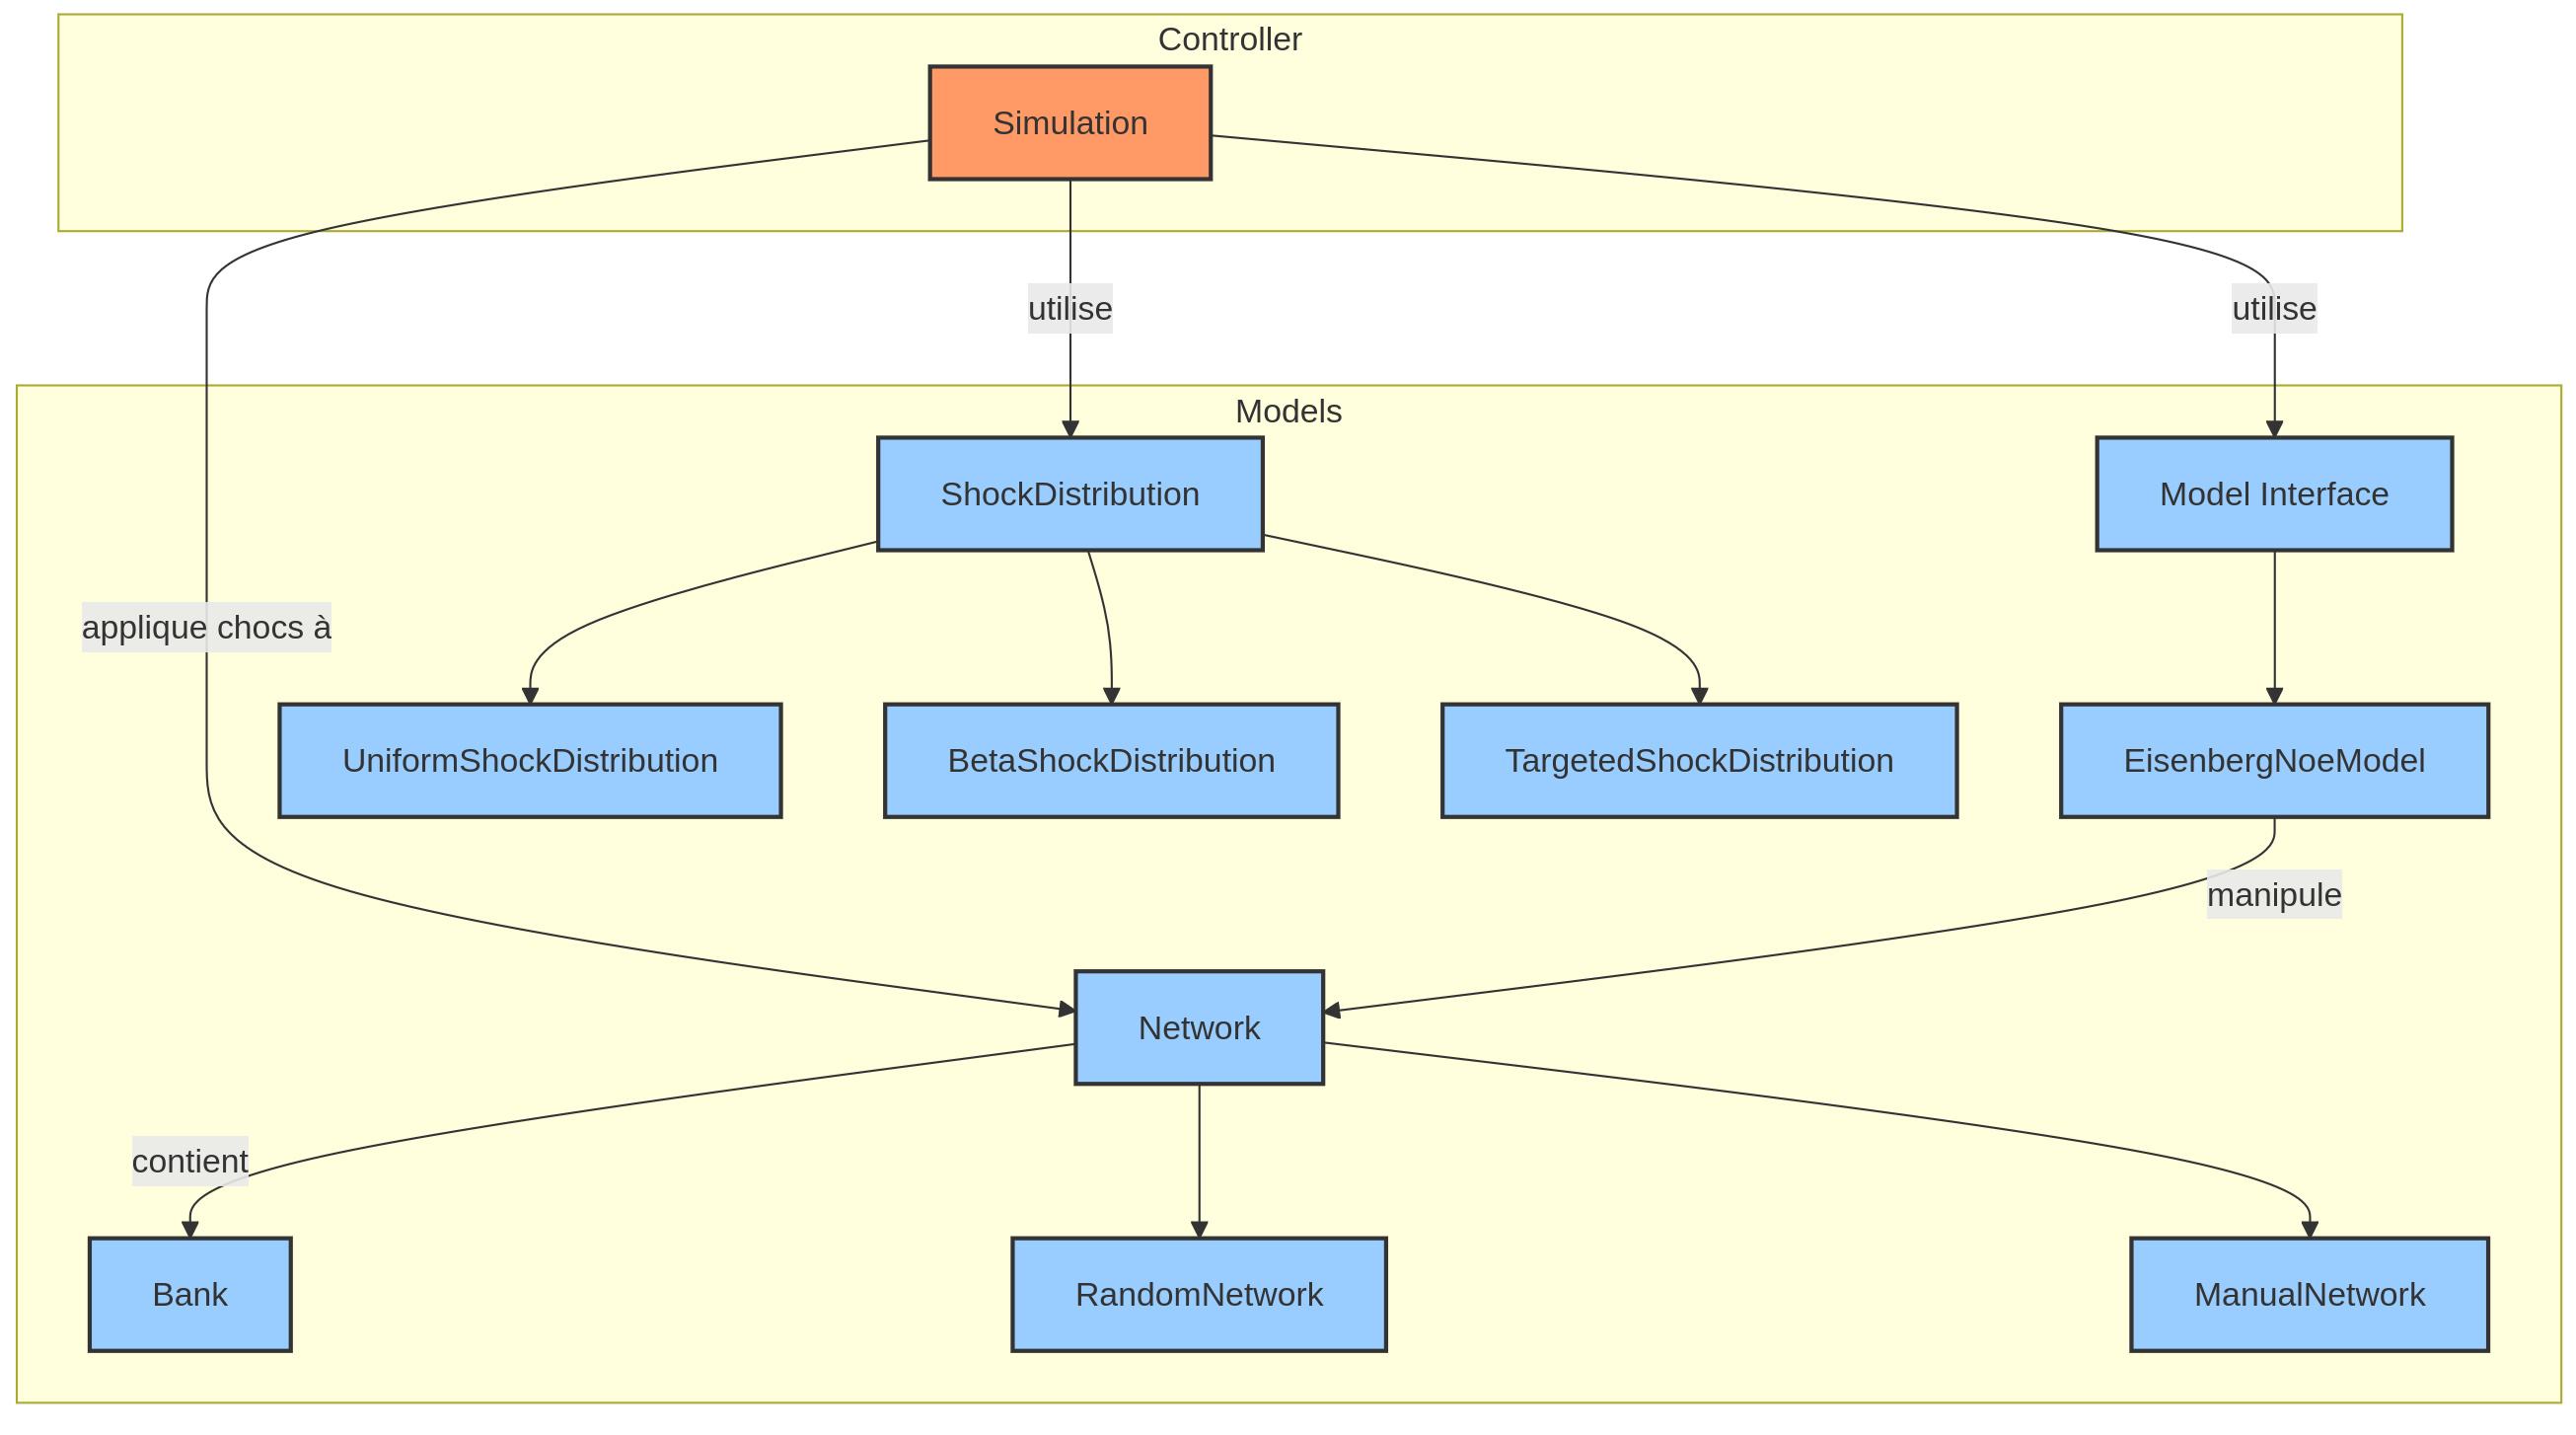
\includegraphics[width=0.8\textwidth]{diagramme uml}

        Architecture MVC facilitant l'extension et la maintenance
    \end{frame}

    \begin{frame}{Équations clés - Algorithme d'Eisenberg-Noe}
        \begin{align}
            \phi(P) &= \min(\bar{P}, \max(0, \Pi^T P + c)) \\
            \bar{P}_i &= [I]_i \\
            \Pi_{ij} &= \frac{[I]_{ij}}{\sum_{k=1}^{n} [I]_{ik} + b_i}
        \end{align}

        \vspace{0.5cm}
        \begin{itemize}
            \item Le vecteur d'équilibre est un point fixe: $\phi(P) = P$
            \item Algorithme itératif: $P^0 = \bar{P}$, $P^{k+1} = \phi(P^k)$
            \item Convergence garantie vers une unique solution
        \end{itemize}
    \end{frame}

    \begin{frame}{Effet de la densité du réseau - Part 2}
        \begin{columns}
            \begin{column}{0.5\textwidth}
                \begin{itemize}
                    \item \textbf{Distinction importante}:
                    \begin{itemize}
                        \item Risque idiosyncratique: dilué par diversification
                        \item Risque systémique: amplifié par l'interconnexion
                    \end{itemize}
                    \vspace{0.1cm}
                    \item Les liens deviennent des canaux de contagion face à un choc global
                \end{itemize}
            \end{column}
            \begin{column}{0.5\textwidth}
                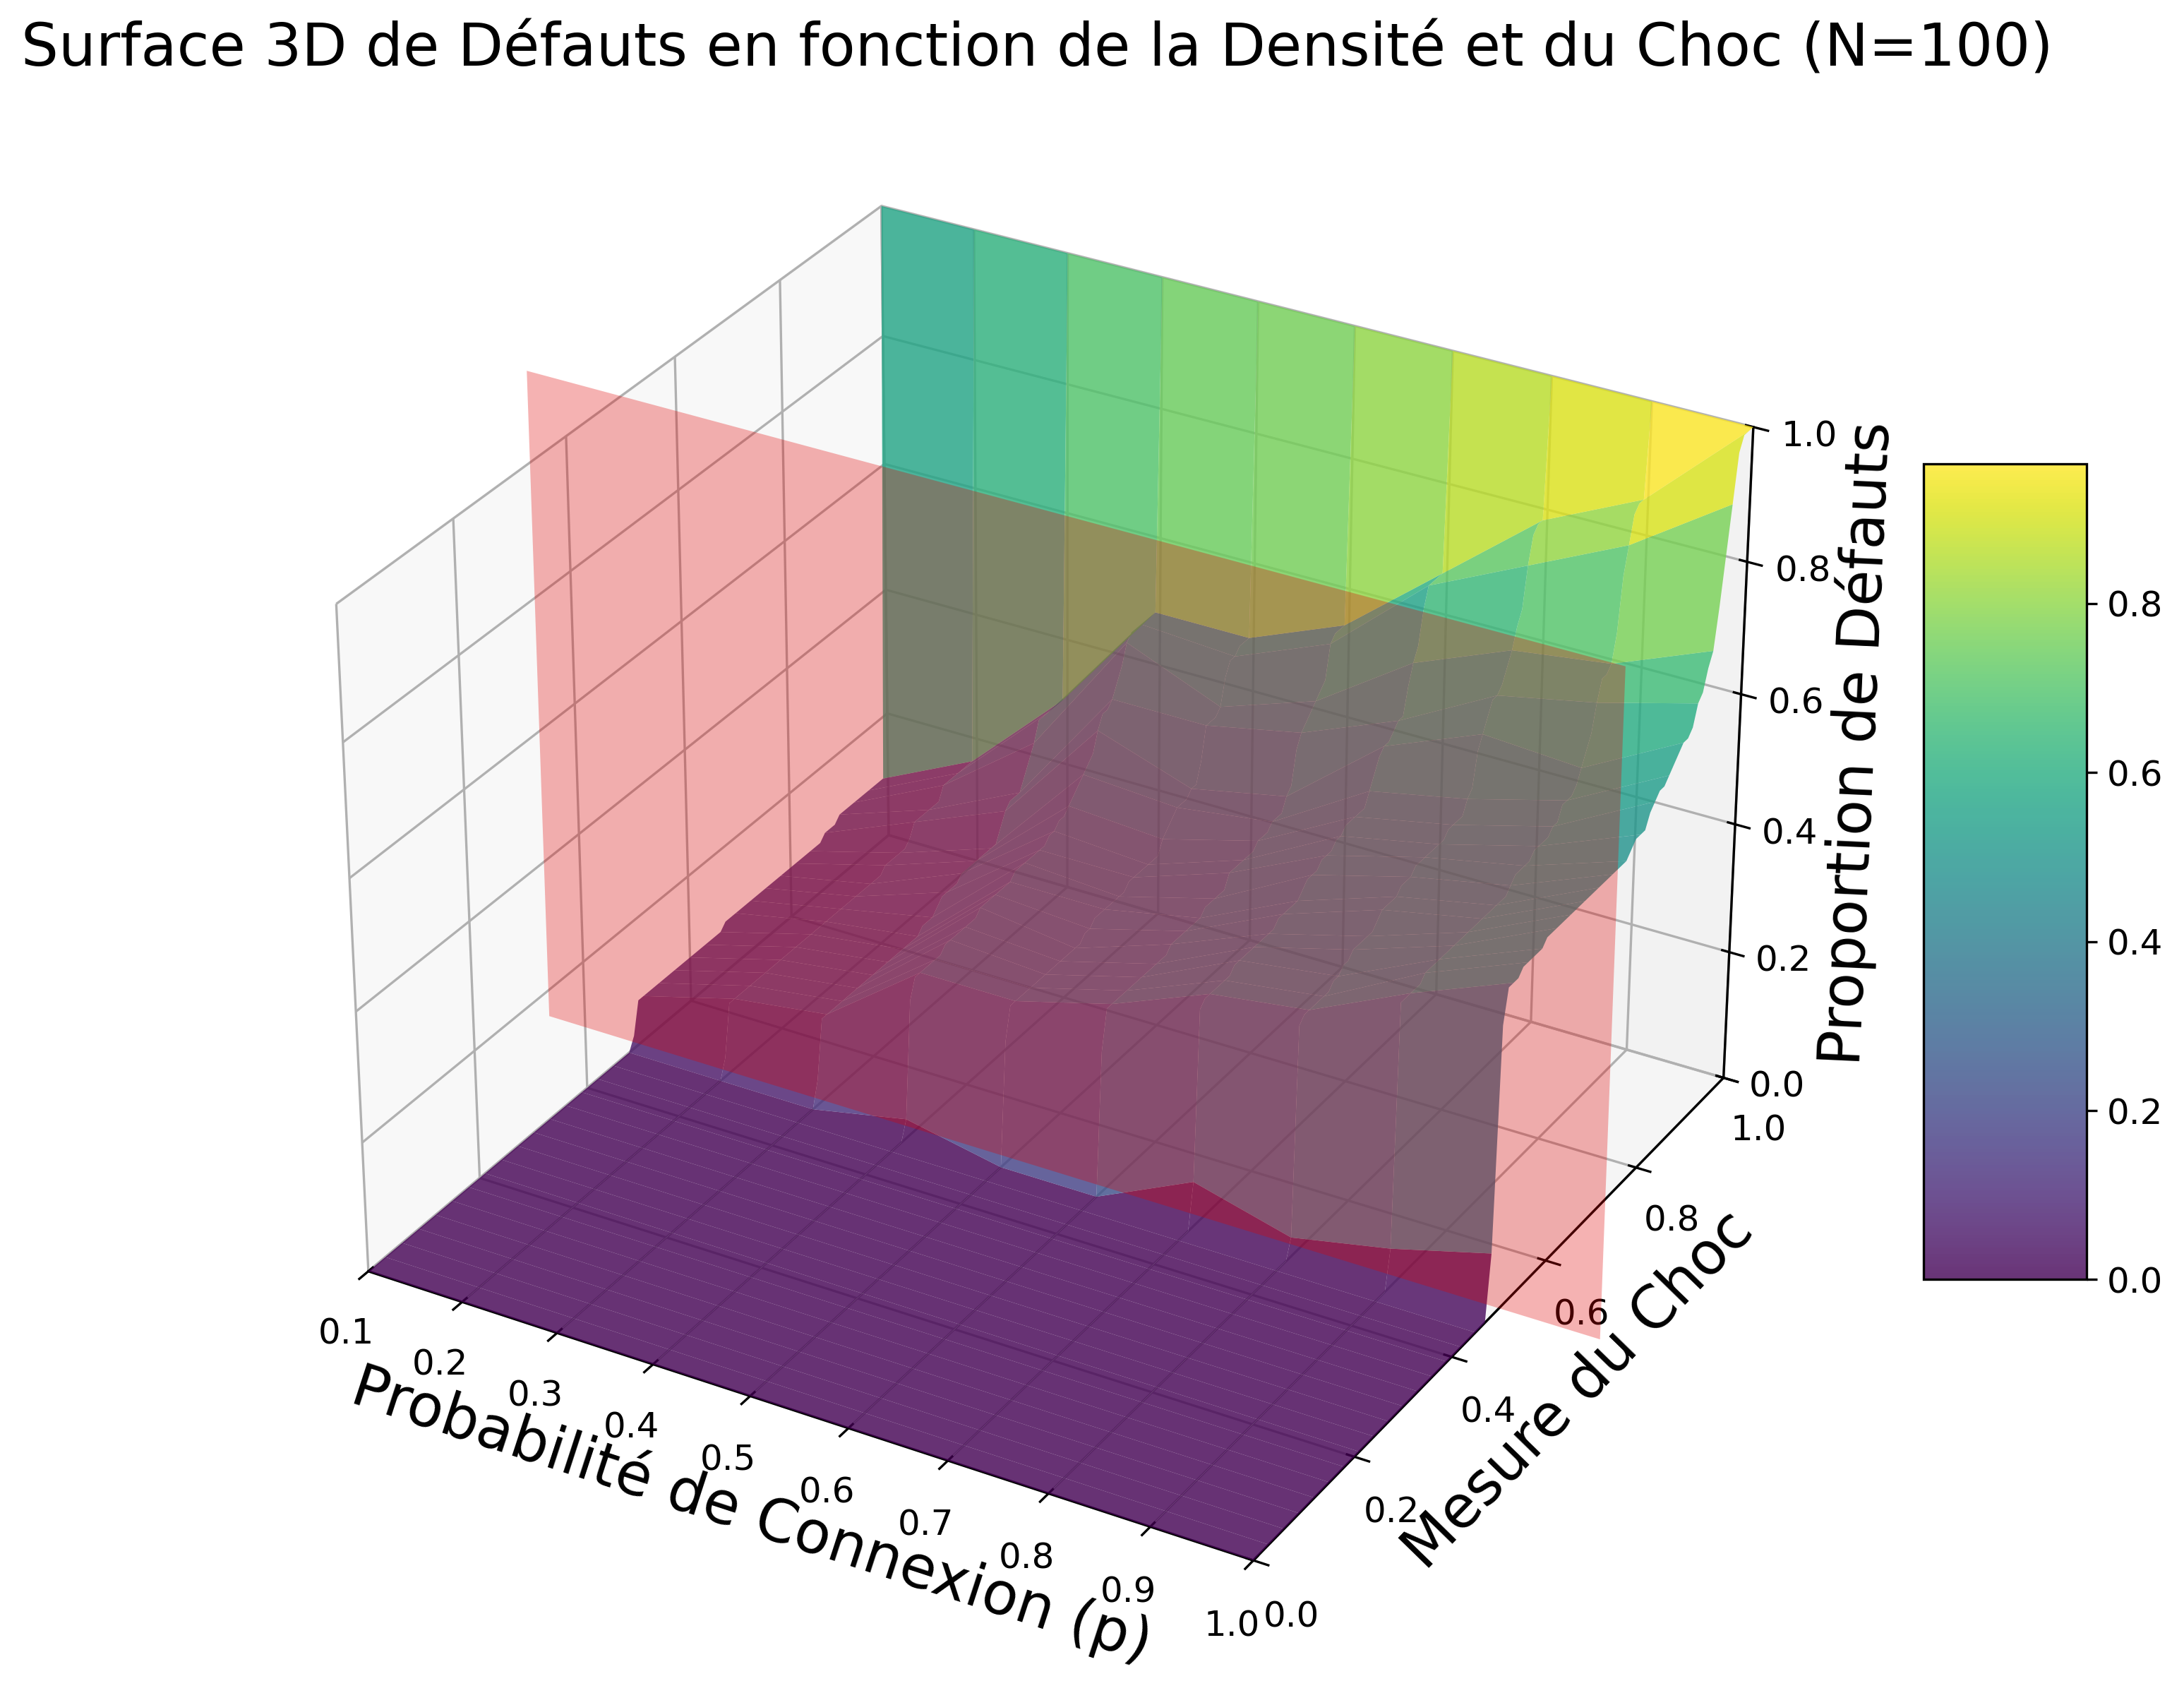
\includegraphics[width=0.9\linewidth]{fig3_3d_prob_shock_default}

                \scriptsize Surface 3D montrant l'interaction entre probabilité de connexion et choc
            \end{column}
        \end{columns}
    \end{frame}



\end{document}